%%%%%%%%%%%%%%%%%%%%%%%%%%%%%%%%%%%%%%%%%
% Programming/Coding Assignment
% LaTeX Template
%
% This template has been downloaded from:
% http://www.latextemplates.com
%
% Original author:
% Ted Pavlic (http://www.tedpavlic.com)
%
% Note:
% The \lipsum[#] commands throughout this template generate dummy text
% to fill the template out. These commands should all be removed when 
% writing assignment content.
%
% This template uses a Perl script as an example snippet of code, most other
% languages are also usable. Configure them in the "CODE INCLUSION 
% CONFIGURATION" section.
%
%%%%%%%%%%%%%%%%%%%%%%%%%%%%%%%%%%%%%%%%%

%----------------------------------------------------------------------------------------
%	PACKAGES AND OTHER DOCUMENT CONFIGURATIONS
%----------------------------------------------------------------------------------------

\documentclass{article}

\usepackage{fancyhdr} % Required for custom headers
\usepackage{lastpage} % Required to determine the last page for the footer
\usepackage{extramarks} % Required for headers and footers
\usepackage[usenames,dvipsnames]{color} % Required for custom colors
\usepackage{graphicx} % Required to insert images
\usepackage{listings} % Required for insertion of code
\usepackage{courier} % Required for the courier font
\usepackage{lipsum} % Used for inserting dummy 'Lorem ipsum' text into the template
\usepackage{csvsimple}

% Margins
\topmargin=-0.45in
\evensidemargin=0in
\oddsidemargin=0in
\textwidth=6.5in
\textheight=9.0in
\headsep=0.25in

\linespread{1.1} % Line spacing

% Set up the header and footer
\pagestyle{fancy}
\lhead{\hmwkAuthorName} % Top left header
\rhead{\hmwkClassShort\ (\hmwkClassInstructor): \hmwkTitle} % Top center head
%\rhead{\firstxmark} % Top right header
%\lfoot{\lastxmark} % Bottom left footer
\cfoot{} % Bottom center footer
\rfoot{Page\ \thepage\ of\ \protect\pageref{LastPage}} % Bottom right footer
\renewcommand\headrulewidth{0.4pt} % Size of the header rule
\renewcommand\footrulewidth{0.4pt} % Size of the footer rule

\setlength\parindent{0pt} % Removes all indentation from paragraphs

%----------------------------------------------------------------------------------------
%	CODE INCLUSION CONFIGURATION
%----------------------------------------------------------------------------------------

\definecolor{MyDarkGreen}{rgb}{0.0,0.4,0.0} % This is the color used for comments
\lstloadlanguages{Perl} % Load Perl syntax for listings, for a list of other languages supported see: ftp://ftp.tex.ac.uk/tex-archive/macros/latex/contrib/listings/listings.pdf
\lstset{language=Perl, % Use Perl in this example
        frame=single, % Single frame around code
        basicstyle=\small\ttfamily, % Use small true type font
        keywordstyle=[1]\color{Blue}\bf, % Perl functions bold and blue
        keywordstyle=[2]\color{Purple}, % Perl function arguments purple
        keywordstyle=[3]\color{Blue}\underbar, % Custom functions underlined and blue
        identifierstyle=, % Nothing special about identifiers                                         
        commentstyle=\usefont{T1}{pcr}{m}{sl}\color{MyDarkGreen}\small, % Comments small dark green courier font
        stringstyle=\color{Purple}, % Strings are purple
        showstringspaces=false, % Don't put marks in string spaces
        tabsize=5, % 5 spaces per tab
        %
        % Put standard Perl functions not included in the default language here
        morekeywords={rand},
        %
        % Put Perl function parameters here
        morekeywords=[2]{on, off, interp},
        %
        % Put user defined functions here
        morekeywords=[3]{test},
       	%
        morecomment=[l][\color{Blue}]{...}, % Line continuation (...) like blue comment
        numbers=left, % Line numbers on left
        firstnumber=1, % Line numbers start with line 1
        numberstyle=\tiny\color{Blue}, % Line numbers are blue and small
        stepnumber=5 % Line numbers go in steps of 5
}

% Creates a new command to include a perl script, the first parameter is the filename of the script (without .pl), the second parameter is the caption
\newcommand{\perlscript}[2]{
\begin{itemize}
\item[]\lstinputlisting[caption=#2,label=#1]{#1.pl}
\end{itemize}
}

%----------------------------------------------------------------------------------------
%	DOCUMENT STRUCTURE COMMANDS
%	Skip this unless you know what you're doing
%----------------------------------------------------------------------------------------

% Header and footer for when a page split occurs within a problem environment
\newcommand{\enterProblemHeader}[1]{
\nobreak\extramarks{#1}{#1 continued on next page\ldots}\nobreak
\nobreak\extramarks{#1 (continued)}{#1 continued on next page\ldots}\nobreak
}

% Header and footer for when a page split occurs between problem environments
\newcommand{\exitProblemHeader}[1]{
\nobreak\extramarks{#1 (continued)}{#1 continued on next page\ldots}\nobreak
\nobreak\extramarks{#1}{}\nobreak
}

\setcounter{secnumdepth}{0} % Removes default section numbers
\newcounter{homeworkProblemCounter} % Creates a counter to keep track of the number of problems

\newcommand{\homeworkProblemName}{}
\newenvironment{homeworkProblem}[1][Problem \arabic{homeworkProblemCounter}]{ % Makes a new environment called homeworkProblem which takes 1 argument (custom name) but the default is "Problem #"
\stepcounter{homeworkProblemCounter} % Increase counter for number of problems
\renewcommand{\homeworkProblemName}{#1} % Assign \homeworkProblemName the name of the problem
\section{\homeworkProblemName} % Make a section in the document with the custom problem count
\enterProblemHeader{\homeworkProblemName} % Header and footer within the environment
}{
\exitProblemHeader{\homeworkProblemName} % Header and footer after the environment
}

\newcommand{\problemAnswer}[1]{ % Defines the problem answer command with the content as the only argument
\noindent\framebox[\columnwidth][c]{\begin{minipage}{0.98\columnwidth}#1\end{minipage}} % Makes the box around the problem answer and puts the content inside
}

\newcommand{\homeworkSectionName}{}
\newenvironment{homeworkSection}[1]{ % New environment for sections within homework problems, takes 1 argument - the name of the section
\renewcommand{\homeworkSectionName}{#1} % Assign \homeworkSectionName to the name of the section from the environment argument
\subsection{\homeworkSectionName} % Make a subsection with the custom name of the subsection
\enterProblemHeader{\homeworkProblemName\ [\homeworkSectionName]} % Header and footer within the environment
}{
\enterProblemHeader{\homeworkProblemName} % Header and footer after the environment
}

%----------------------------------------------------------------------------------------
%	NAME AND CLASS SECTION
%----------------------------------------------------------------------------------------

\newcommand{\hmwkTitle}{Project\ Deliverable\ \#3} % Assignment title
\newcommand{\hmwkDueDate}{Tuesday,\ June\ 3$^{rd}$,\ 2014} % Due date
\newcommand{\hmwkClass}{CS-322\ Introduction\ to\ Database\ Systems} % Course/class
\newcommand{\hmwkClassShort}{CS-322}
\newcommand{\hmwkClassTime}{09:15am} % Class/lecture time
\newcommand{\hmwkClassInstructor}{Anastasia Ailamaki} % Teacher/lecturer
\newcommand{\hmwkAuthorFullName}{Elise KLAY, Maxime AMEHO, Baptiste VINH MAU} % Your name
\newcommand{\hmwkAuthorName}{Klay, Ameho, Vinh Mau} % Your name
\newcommand{\hmwkGroup}{Group 24}
%----------------------------------------------------------------------------------------
%	TITLE PAGE
%----------------------------------------------------------------------------------------

\title{
\vspace{2in}
\textmd{\textbf{\hmwkClass}}\\
\textmd{\textbf{\hmwkTitle}}\\
\normalsize\vspace{0.1in}\small{Due\ on\ \hmwkDueDate}\\
\vspace{0.1in}
\vspace{2.5in}
}

\author{\textbf{\hmwkGroup} \\ \textbf{\hmwkAuthorName}}
\date{} % Insert date here if you want it to appear below your name

%----------------------------------------------------------------------------------------

\begin{document}

\maketitle
\begin{center}

\includegraphics[width=0.4\columnwidth]{EPFL} % Example image
\end{center}

%----------------------------------------------------------------------------------------
%	TABLE OF CONTENTS
%----------------------------------------------------------------------------------------

%\setcounter{tocdepth}{1} % Uncomment this line if you don't want subsections listed in the ToC

\newpage
%\tableofcontents
%\newpage

%----------------------------------------------------------------------------------------
%	REPORT
%----------------------------------------------------------------------------------------

% To have just one problem per page, simply put a \clearpage after each problem
\section*{ER model for music database}
\problemAnswer{
\begin{center}
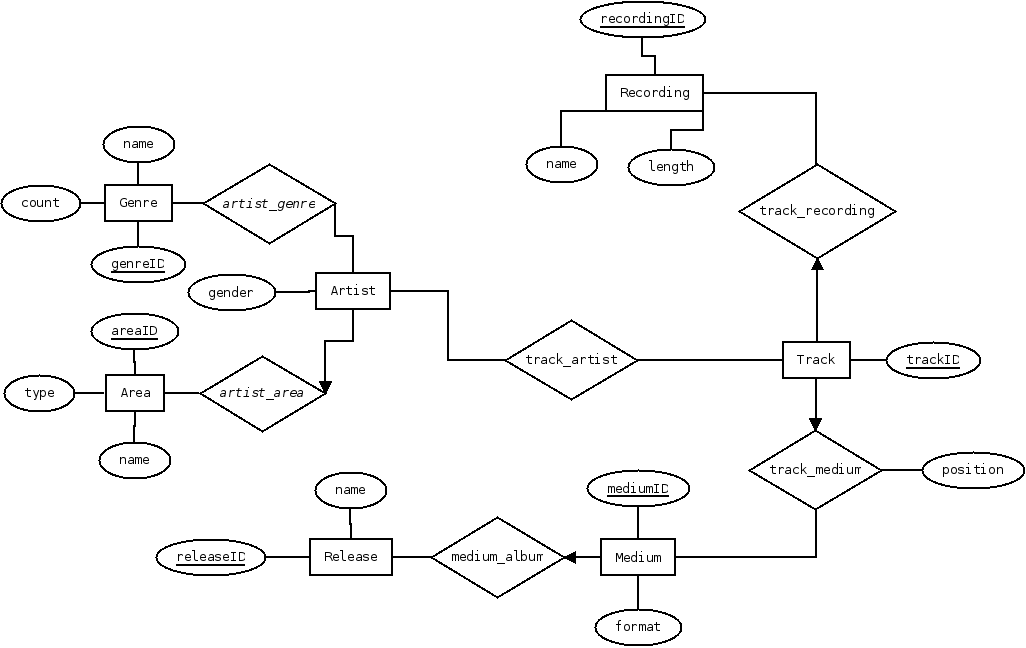
\includegraphics[width=1\columnwidth]{er} % Example image
\end{center}
}
\section*{SQL DDL code for table creations}
\lstinputlisting[language=SQL]{../scripts/entities.sql}{SQL script for entities table creation}
\\
\lstinputlisting[language=SQL]{../scripts/relations.sql}{SQL script for relations table creation}

\section*{Design choices \& data constraints}
\problemAnswer{
There are three main concepts in our music database : \textbf{Song}, \textbf{Artist} and \textbf{Album}. Both Song and Album were divided between 
their descriptive data (\textbf{Recording, Release}) and their physical incarnation (\textbf{Track, Medium}). 
Since data is often incomplete, most of the entities 'can be related' but do not have to.
We put a NOT NULL constraint on most of the name attributes of the entities, with the exception of \textbf{Recording} for the reason just stated. Since they are not required fields to describe 
music, they should have a valid name when they are in fact used.

\begin{itemize}
  \item A \textbf{Track} is related to:
    \begin{description}
	\item[Recording: ] A track can be a physical incarnation of a known recording.
      \item[Artist: ] A track can exist without known artists, but can also have several artists to describe collaborations.
      \item[Medium: ] A track can be recorded on some medium. Their relation is characterized by the track position on the medium.
    \end{description}

  \item An \textbf{Artist} is defined by a:
    \begin{description}
      \item[Genre: ] A genre can regroup multiple artists,
      whereas an artist can be difficult to define as catering to a specific genre, or crossing boundaries between genres nullifying the need for a constraint. We kept the count attribute, 
      choosing small update costs over on-demand higher computation costs. 
      \item[Area: ] An artist's location can be pinpointed to a specific creation grounds, hence can be expressed by a foreign key constraint. But several artists can be compelled 
      to share their musical feelings in the same studio.
    \end{description} 

  \item A \textbf{Release} is the logical aggregation of songs, labeled by a title, and can be recorded on multiple mediums. 
  Conversely, a medium identifies a singular recording of an album, enforced by a foreign key constraint.
\end{itemize}

The integrity of the count attribute in \textbf{Genre}, are not guaranteed by the table creation. It will
later be enforced later on by the import and delete data commands.

}

\section*{Design changes from deliverable 1}
We removed all of our 'at least one' constraints to facilitate the import of new data. For the same reason, we also changed our model to be closer to the given data, so that 
one can easily add any information into the database and not just track-related information like we initially had in mind. That is, in our first model, everything 
had to be related to a track to be relevant but now every entities are independent. 

\section*{Data import }
After having quite a lot of trouble trying to import the data on the oracle server, we decided to use a local database
instead. We used SQLite to handle this database.


\section*{Interface}
%----------------------------------------------------------------------------------------
We chose to use Python to design the software with the SQLAlchemy API to interface with the database. 
Therefore we used PyQt5 to design the GUI itself providing clean and practical tools. 
SQLAlchemy offers a very useful model as it reflects accurately the actual database schema and makes it easier to map the data to the Model/View offered by Qt.
\\
\problemAnswer
{
\begin{center}
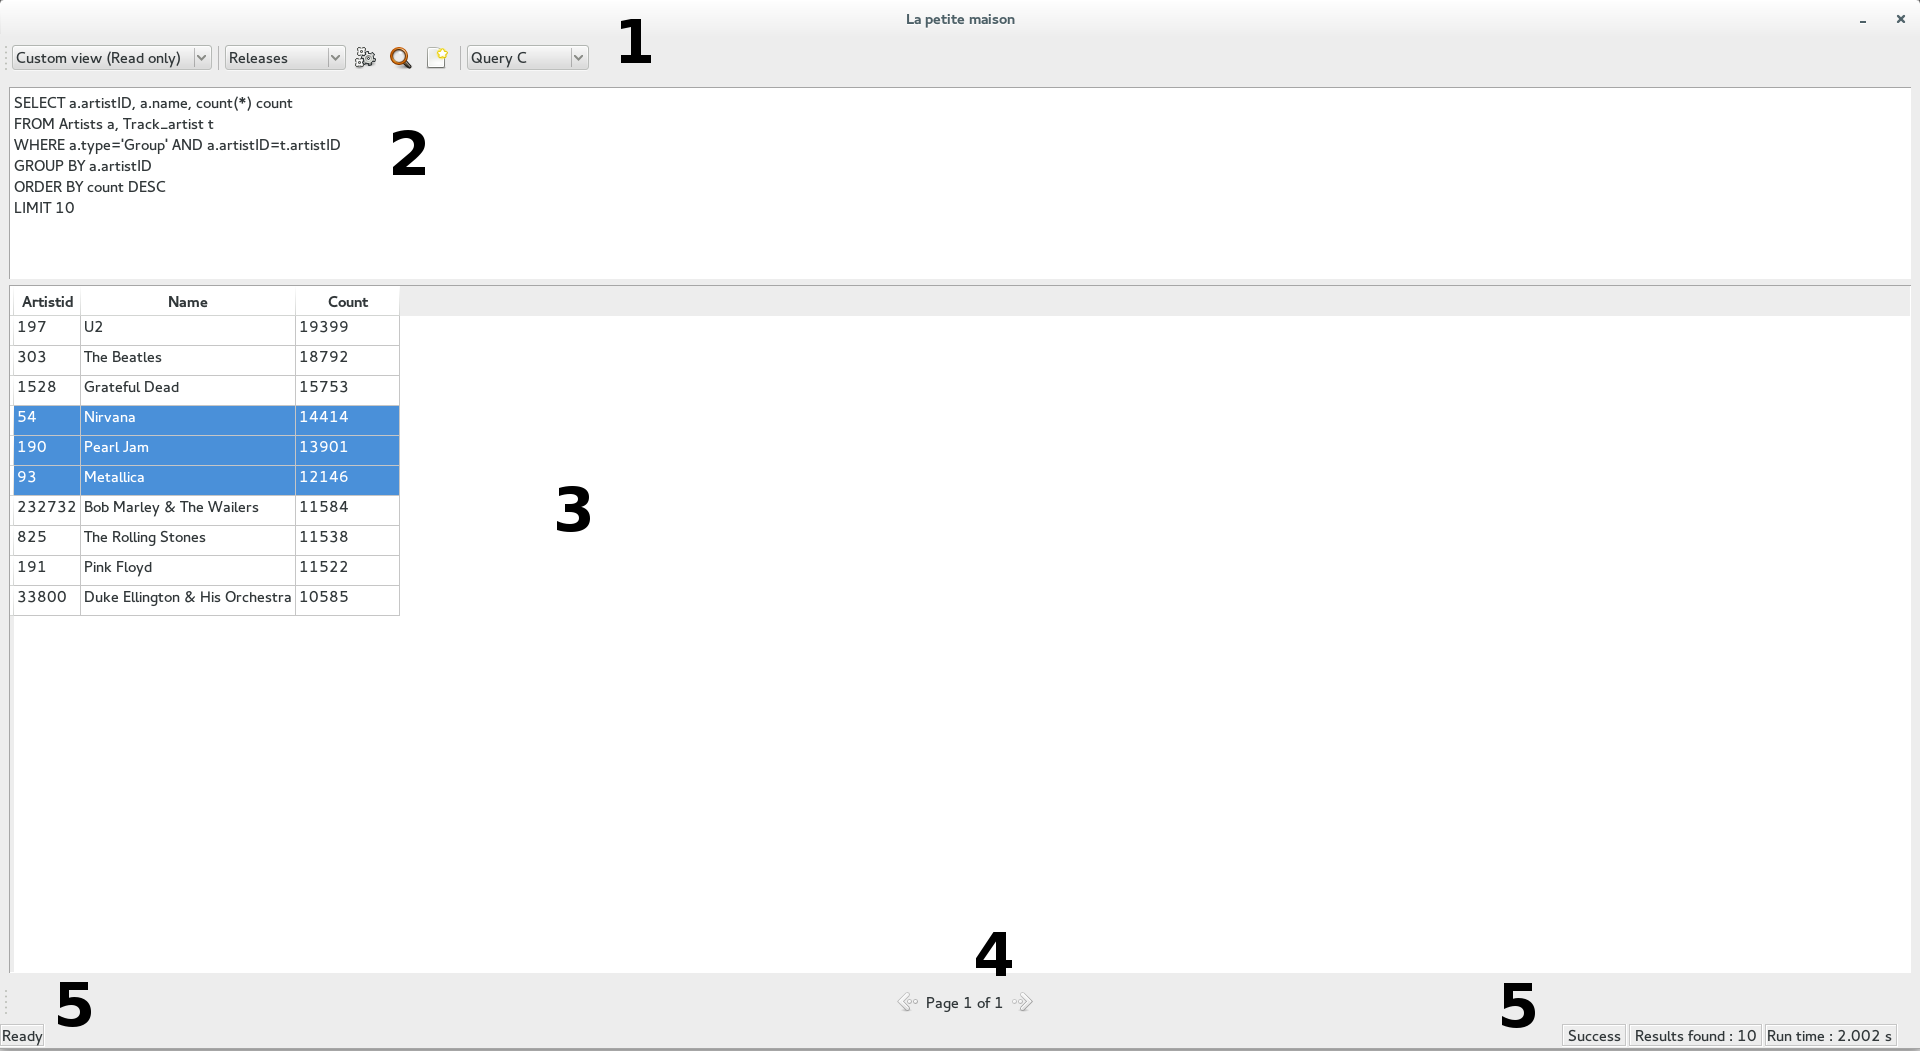
\includegraphics[width=1\columnwidth]{interface.png}
\end{center}
}
\bigskip

Our interface allows the user to write their own queries, while providing them with friendly ways to build simple queries to navigate through the database, to edit or delete records and 
to add new ones. The above picture shows our interface, after loading and running query C.
The permissions and access to the different elements of the functionnality is handled through modes. Though we did not have the
time to do it, this could easily be associated with user permissions. We have four different modes, which are a cross product
between table view (tables' columns as in database) or custom view, and read/write or write only.
\begin{itemize}
\item 1 : The upper tool bar offers most of the available functions to create and run queries. From left to right we have the mode selection, the table selection, 
the buttons to run the current query, to search for keywords in the current results and to add a new record to the current table (only in table view) and lastly
the list of the loadable existing queries. A pending query can be canceled by clicking 
a second time on the run button. 
\item 2 : The query is displayed in a text box. It can only be edited in custom mode. 
\item 3 : The results of the last query are shown in a table. 
\item 4 : The navigation tool bar allows user to switch between result pages.
\item 5 : The status bar gives feedback about the queries' runs. On the left, the status (ready or query pending) is given. On the right, if the last request was successful, 
how many results it found and its run time. 
\end{itemize}
Right click on the table provides a contextual menu where the user can choose to edit or delete the selected
entries (in view mode) or to make some follow up queries depending on the selected field. So for instance if we select 
Nirvana, Pearl Jam and Metallica in our table and right click, we can then show all releases featuring those artists.
\bigskip

\problemAnswer
{

\begin{center}
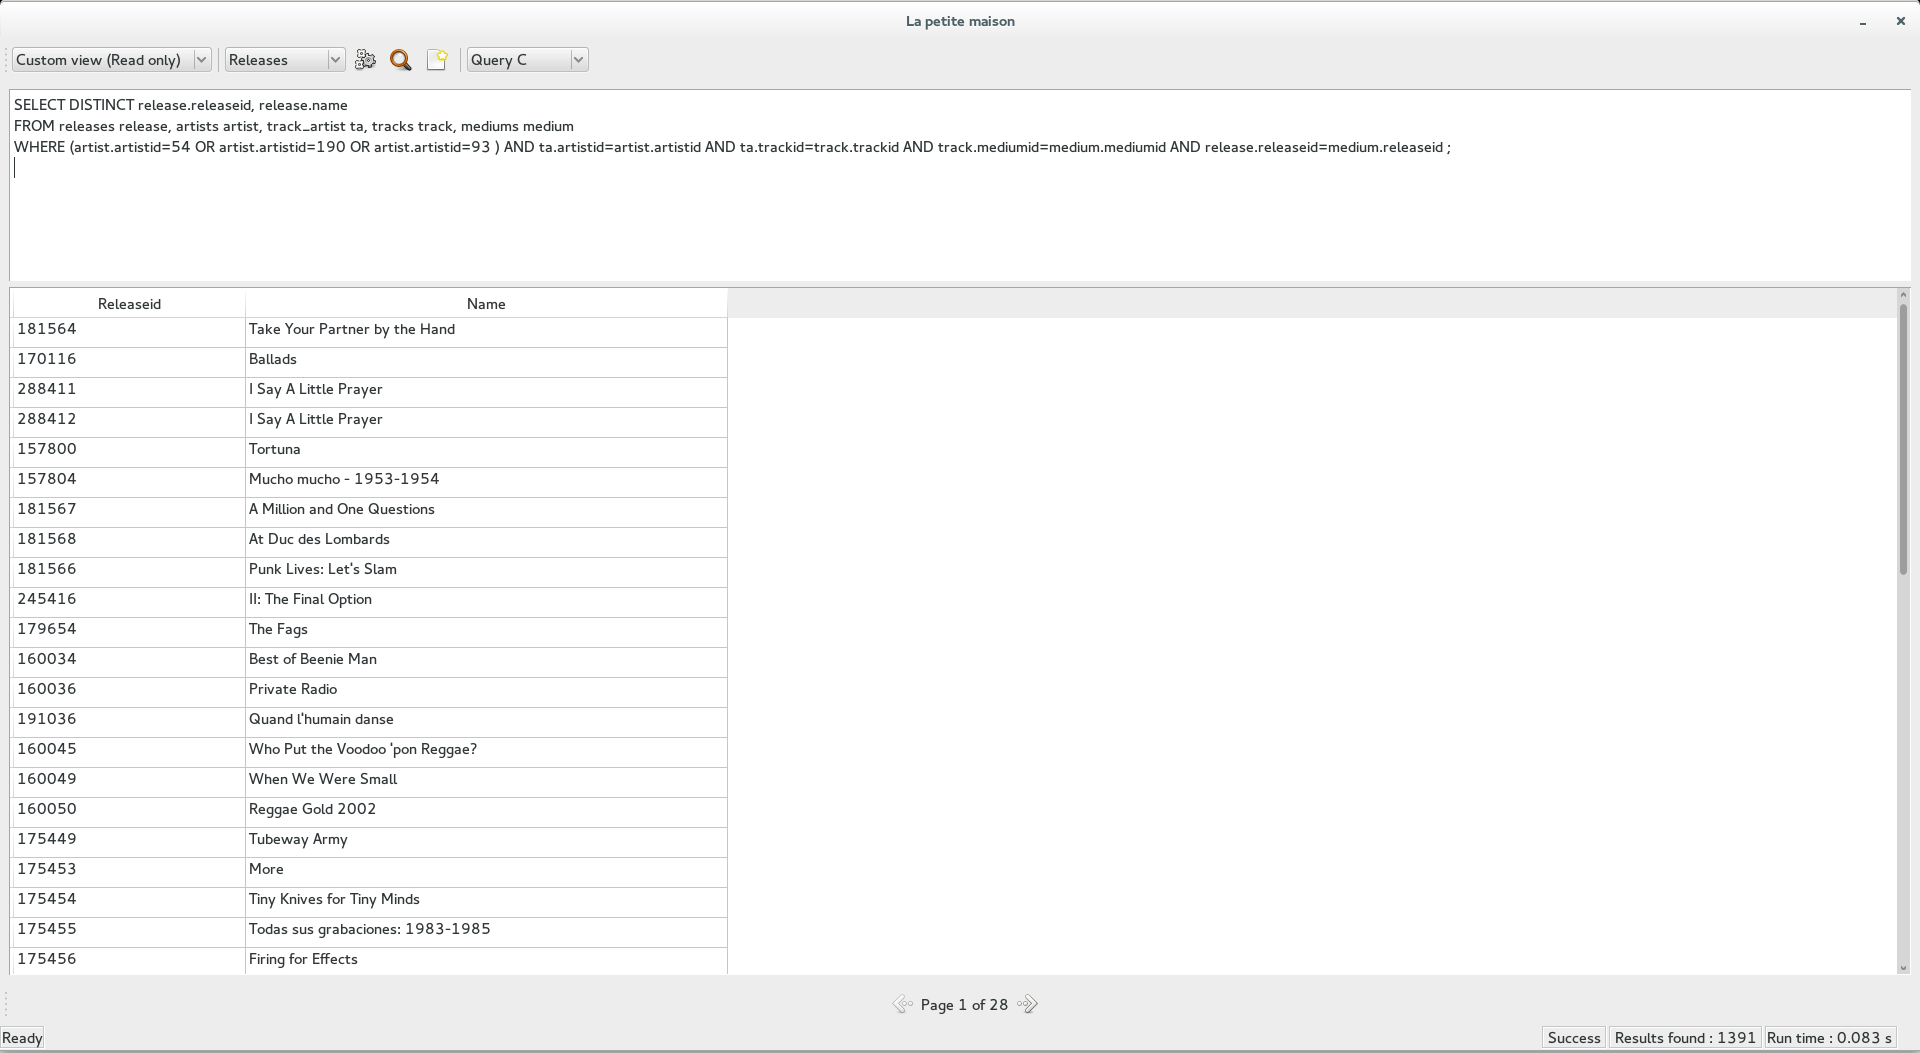
\includegraphics[width=1\columnwidth]{followup.png}
\end{center}
}
\bigskip

The update, search and insert queries are handled by pop up dialogs, providing tables to be filled which are then turned into queries. For instance, we can add a new artist.

\bigskip
\problemAnswer
{
\begin{center}
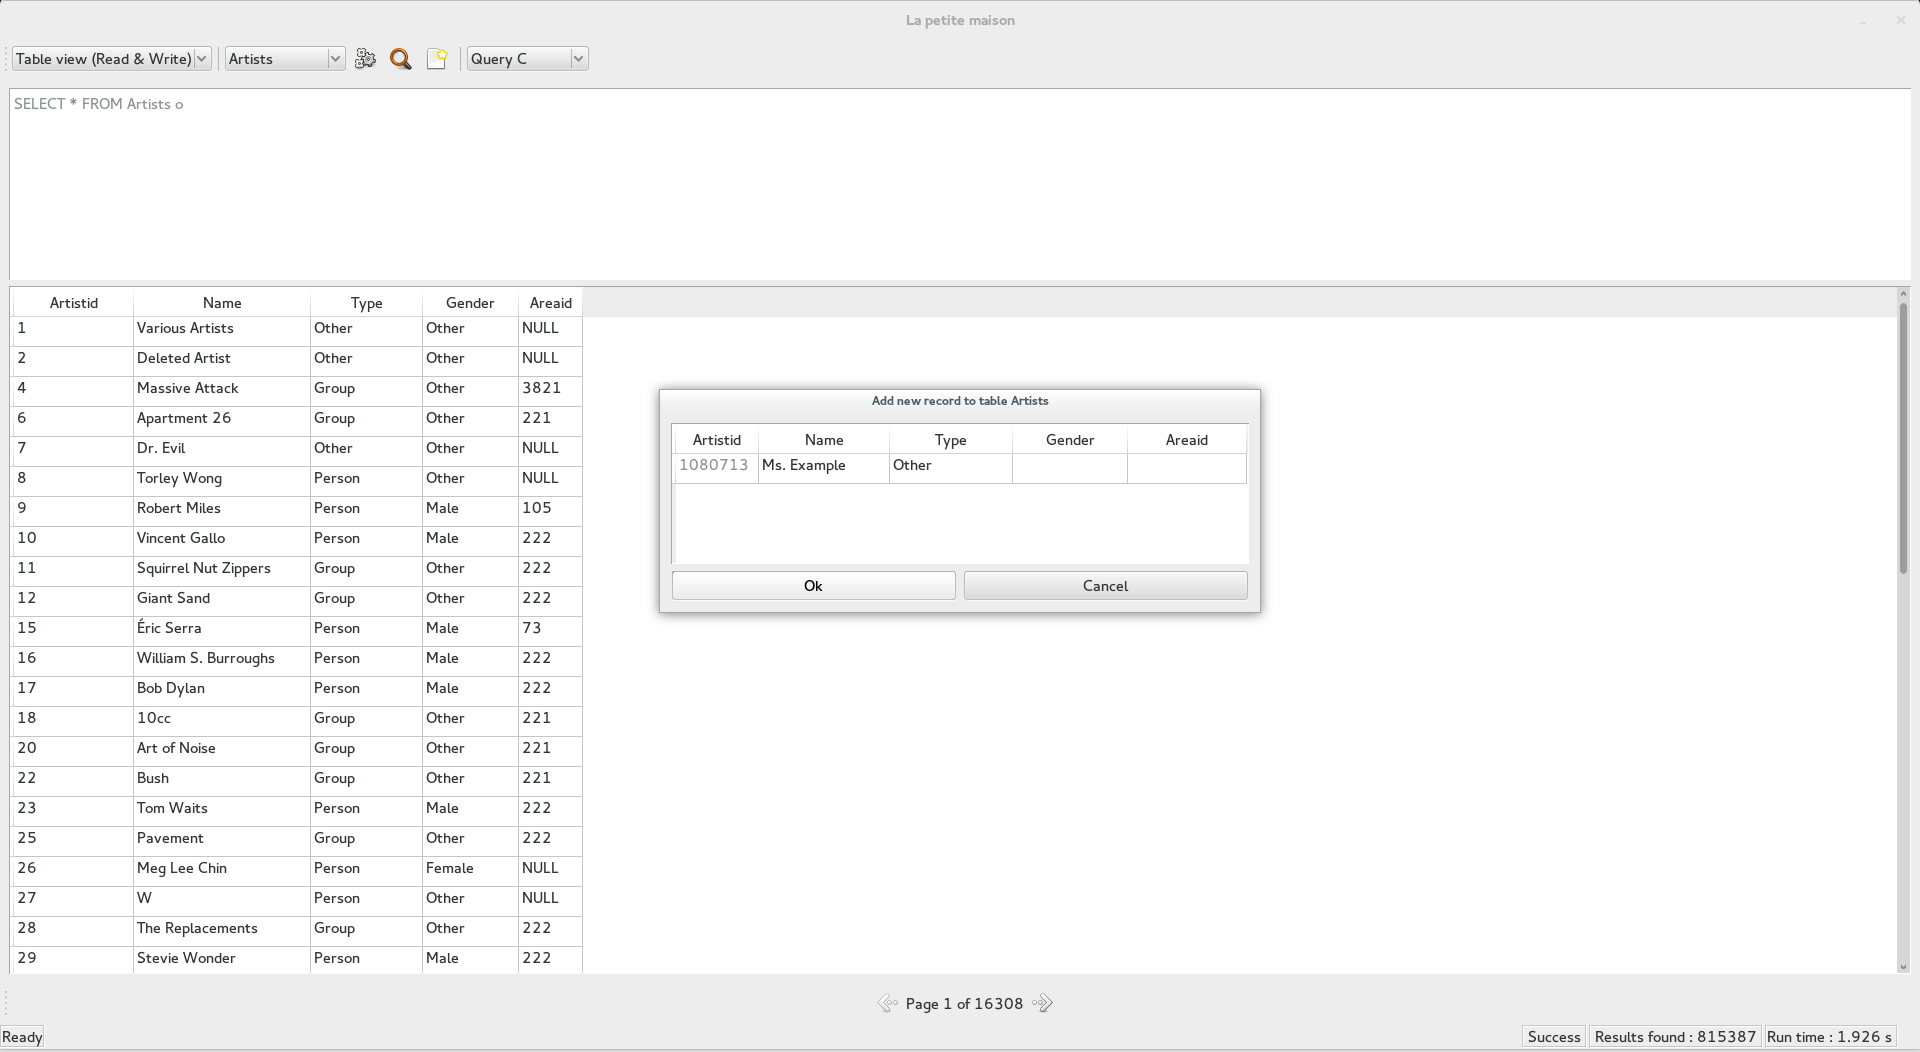
\includegraphics[width=1\columnwidth]{addrecord.png}
\end{center}
}

\section*{Queries \& performance analysis}
As we had chosen to work using Oracle DB our queries were first written using this dialect. Due to issues related to the heavy concurrent usage of the server we later elected to transfer to a local database built using SQLite. However failure to communicate, and an improvable work distribution lead to gaps in the translation to SQLite. We therefore present in this report both versions of the queries.

\subsection*{SQL Queries}

\subsection*{SQLite}
\lstinputlisting[language=SQL]{../scripts/A.sql}{SQL script for query A} \\
\lstinputlisting[language=SQL]{../scripts/B.sql}{SQL script for query B} \\
\lstinputlisting[language=SQL]{../scripts/C.sql}{SQL script for query C} \\
\lstinputlisting[language=SQL]{../scripts/D.sql}{SQL script for query D} \\
\lstinputlisting[language=SQL]{../scripts/E.sql}{SQL script for query E} \\
\lstinputlisting[language=SQL]{../scripts/F.sql}{SQL script for query F} \\
\lstinputlisting[language=SQL]{../scripts/G.sql}{SQL script for query G} \\
\lstinputlisting[language=SQL]{../scripts/H.sql}{SQL script for query H} \\
\lstinputlisting[language=SQL]{../scripts/I.sql}{SQL script for query I} \\
\lstinputlisting[language=SQL]{../scripts/J.sql}{SQL script for query J} \\
\lstinputlisting[language=SQL]{../scripts/K.sql}{SQL script for query K} \\
\lstinputlisting[language=SQL]{../scripts/L.sql}{SQL script for query L} \\
\lstinputlisting[language=SQL]{../scripts/M.sql}{SQL script for query M} \\
\lstinputlisting[language=SQL]{../scripts/N.sql}{SQL script for query N} \\
\lstinputlisting[language=SQL]{../scripts/O.sql}{SQL script for query O} \\
\lstinputlisting[language=SQL]{../scripts/P.sql}{SQL script for query P} \\
\lstinputlisting[language=SQL]{../scripts/Q.sql}{SQL script for query Q} \\
\lstinputlisting[language=SQL]{../scripts/R.sql}{SQL script for query R} \\
\lstinputlisting[language=SQL]{../scripts/S.sql}{SQL script for query S} \\


\subsubsection*{Oracle}
\lstinputlisting[language=SQL]{../scripts/Oracle/A.sql}{SQL script for query A} \\
\lstinputlisting[language=SQL]{../scripts/Oracle/B.sql}{SQL script for query B} \\
\lstinputlisting[language=SQL]{../scripts/Oracle/C.sql}{SQL script for query C} \\
\lstinputlisting[language=SQL]{../scripts/Oracle/D.sql}{SQL script for query D} \\
\lstinputlisting[language=SQL]{../scripts/Oracle/E.sql}{SQL script for query E} \\
\lstinputlisting[language=SQL]{../scripts/Oracle/F.sql}{SQL script for query F} \\
\lstinputlisting[language=SQL]{../scripts/Oracle/G.sql}{SQL script for query G} \\
\lstinputlisting[language=SQL]{../scripts/Oracle/H.sql}{SQL script for query H} \\
\lstinputlisting[language=SQL]{../scripts/Oracle/I.sql}{SQL script for query I} \\
\lstinputlisting[language=SQL]{../scripts/Oracle/J.sql}{SQL script for query J} \\
\lstinputlisting[language=SQL]{../scripts/Oracle/K.sql}{SQL script for query K} \\
\lstinputlisting[language=SQL]{../scripts/Oracle/L.sql}{SQL script for query L} \\
\lstinputlisting[language=SQL]{../scripts/Oracle/M.sql}{SQL script for query M} \\
\lstinputlisting[language=SQL]{../scripts/Oracle/N.sql}{SQL script for query N} \\
\lstinputlisting[language=SQL]{../scripts/Oracle/O.sql}{SQL script for query O} \\
\lstinputlisting[language=SQL]{../scripts/Oracle/P.sql}{SQL script for query P} \\
\lstinputlisting[language=SQL]{../scripts/Oracle/Q.sql}{SQL script for query Q} \\
\lstinputlisting[language=SQL]{../scripts/Oracle/R.sql}{SQL script for query R} \\
\lstinputlisting[language=SQL]{../scripts/Oracle/S.sql}{SQL script for query S} \\

\subsection*{Run Time}
We display here the run times in seconds for each query, as given to us by the sqlite timer function. Real time corresponds to the time elapsed from start to end of the query, while user and system times correspond to CPU time spend respectively in user and kernel mode. The execution time of the query on the CPU would then equal the sum of both these terms.
\bigskip
\\
\csvautotabular{runtime.csv}
\subsection*{On the necessity of indexes}
We chose queries I, K and M for our analysis. 
\\

\end{document}
